\documentclass[11pt]{article}
% Shared style for BELAND-PLUS academic revision R3
% Typography: Latin Modern (the canonical scalable Computer Modern family).
\usepackage[T1]{fontenc}
\usepackage[utf8]{inputenc}
\usepackage{lmodern}
\usepackage{microtype}
\usepackage{amsmath,amssymb,mathtools,bm}
\usepackage{booktabs,threeparttable,longtable,tabularx,array,multirow,makecell}
\usepackage{graphicx,adjustbox}
\usepackage{caption,subcaption}
\usepackage{tikz}
\usetikzlibrary{arrows.meta,positioning,fit,calc,backgrounds,matrix,decorations.pathreplacing,shapes.geometric}
\usepackage{pgfplots}
\pgfplotsset{compat=1.18}
\usepackage{xcolor}
\usepackage{geometry}
\geometry{margin=1in,headheight=15pt,footskip=30pt}
\usepackage{setspace}
\setstretch{1.10}
\usepackage{enumitem}
\setlist[itemize]{leftmargin=1.55em,itemsep=0.18em,topsep=0.35em,parsep=0pt}
\setlist[enumerate]{leftmargin=1.8em,itemsep=0.18em,topsep=0.35em,parsep=0pt}
\usepackage{titlesec}
\titleformat{\section}{\large\bfseries}{\thesection}{0.75em}{}
\titleformat{\subsection}{\normalsize\bfseries}{\thesubsection}{0.65em}{}
\titleformat{\subsubsection}{\normalsize\itshape}{\thesubsubsection}{0.55em}{}
\titlespacing*{\section}{0pt}{2.0ex plus .4ex minus .2ex}{0.9ex}
\titlespacing*{\subsection}{0pt}{1.55ex plus .3ex minus .2ex}{0.65ex}
\titlespacing*{\subsubsection}{0pt}{1.1ex plus .2ex minus .2ex}{0.45ex}
\usepackage{fancyhdr}
\pagestyle{fancy}
\fancyhf{}
\fancyhead[L]{\footnotesize\itshape Hurricane Ida and public emergency-service observability}
\fancyhead[R]{\footnotesize BELAND-PLUS}
\fancyfoot[C]{\thepage}
\renewcommand{\headrulewidth}{0.35pt}
\renewcommand{\footrulewidth}{0pt}
\usepackage[round,authoryear]{natbib}
\usepackage{hyperref}
\usepackage[nameinlink,noabbrev]{cleveref}
\usepackage{xurl}
\urlstyle{same}
\usepackage{csquotes}
\usepackage{listings}
\usepackage{tcolorbox}
\tcbuselibrary{breakable,skins}
\usepackage{float}
\usepackage[section]{placeins}
\usepackage{siunitx}
\sisetup{detect-all,group-separator={,},group-minimum-digits=4,table-number-alignment=center}
\usepackage{pdflscape}
\usepackage{etoolbox}

\definecolor{BelandBlue}{HTML}{183A5A}
\definecolor{BelandBlueLight}{HTML}{EAF0F5}
\definecolor{BelandOrange}{HTML}{B5652A}
\definecolor{BelandRed}{HTML}{9E3D36}
\definecolor{BelandGray}{HTML}{4B5563}
\definecolor{BelandLightGray}{HTML}{F4F5F7}
\definecolor{BelandGreen}{HTML}{2E6F64}
\definecolor{BelandGold}{HTML}{A47A24}

\hypersetup{
  colorlinks=true,
  linkcolor=BelandBlue,
  citecolor=BelandBlue,
  urlcolor=BelandBlue,
  pdfborder={0 0 0}
}

\newcommand{\Jzerozero}{J_{00}}
\newcommand{\Jzeroone}{J_{01}}
\newcommand{\Jonezero}{J_{10}}
\newcommand{\Joneone}{J_{11}}
\newcommand{\E}{\mathrm{E}}
\newcommand{\R}{\mathrm{R}}
\newcommand{\Prob}{\Pr}
\newcommand{\Ida}{\mathrm{Ida}}
\newcommand{\Iset}{\mathcal{I}}
\newcommand{\Mset}{\mathfrak{M}}
\newcommand{\Xset}{\mathcal{X}}
\newcommand{\supp}{\operatorname{supp}}
\newcommand{\diam}{\operatorname{diam}}
\newcommand{\argmin}{\operatorname*{arg\,min}}
\newcommand{\argmax}{\operatorname*{arg\,max}}
\newcommand{\ind}{\mathbf{1}}
\newcommand{\Rset}{\mathbb{R}}
\newcommand{\Nset}{\mathbb{N}}
\newcommand{\abs}[1]{\left|#1\right|}
\newcommand{\norm}[1]{\left\lVert#1\right\rVert}
\newcommand{\given}{\,|\,}

\newtcolorbox{plainbox}[1][]{
  enhanced,breakable,colback=BelandBlueLight,colframe=BelandBlue,
  boxrule=0.55pt,arc=1.5mm,left=2.7mm,right=2.7mm,top=1.8mm,bottom=1.8mm,#1}
\newtcolorbox{resultbox}[1][]{
  enhanced,breakable,colback=BelandLightGray,colframe=BelandGray,
  boxrule=0.5pt,arc=1.5mm,left=2.7mm,right=2.7mm,top=1.8mm,bottom=1.8mm,#1}
\newtcolorbox{warningbox}[1][]{
  enhanced,breakable,colback=white,colframe=BelandOrange,
  boxrule=0.65pt,arc=1.5mm,left=2.7mm,right=2.7mm,top=1.8mm,bottom=1.8mm,#1}
\newtcolorbox{definitionbox}[1][]{
  enhanced,breakable,colback=white,colframe=BelandBlue!70,
  boxrule=0.45pt,arc=1.2mm,left=2.5mm,right=2.5mm,top=1.5mm,bottom=1.5mm,#1}

\captionsetup{font=small,labelfont=bf,labelsep=period,skip=5pt,justification=raggedright,singlelinecheck=false}
\renewcommand{\arraystretch}{1.18}
\setlength{\tabcolsep}{5pt}
\setlength{\parindent}{1.35em}
\setlength{\parskip}{0pt}
\setlength{\emergencystretch}{2em}
\raggedbottom

\lstdefinestyle{belandcode}{
  basicstyle=\ttfamily\footnotesize,
  backgroundcolor=\color{BelandLightGray},
  frame=single,
  rulecolor=\color{BelandGray!45},
  breaklines=true,
  breakatwhitespace=false,
  columns=fullflexible,
  keepspaces=true,
  showstringspaces=false,
  xleftmargin=0.5em,
  xrightmargin=0.5em,
  aboveskip=0.7em,
  belowskip=0.7em
}
\lstset{style=belandcode}

\newcommand{\notclaim}[1]{\textit{This does not identify #1.}}
\newcommand{\pp}{percentage points}
\newcommand{\keywords}[1]{\par\noindent\textbf{Keywords:} #1}
\newcommand{\jel}[1]{\par\noindent\textbf{JEL codes:} #1}

\AtBeginEnvironment{tabular}{\small}
\AtBeginEnvironment{tabularx}{\small}
\AtBeginEnvironment{longtable}{\small}

\fancyhead[L]{\footnotesize\itshape Public CAD is not operational ground truth}

\title{\vspace{-1.7em}\textbf{Public CAD Is Not Operational Ground Truth}\\[0.35em]
\large Hurricane Ida and the Measurement of Police Responsiveness}
\author{}
\date{24 August 2026\\[0.2em]\small Paper R13.0 \quad Results R12}

\begin{document}
\maketitle
\thispagestyle{plain}
\vspace{-1.3em}

\begin{plainbox}[title=Abstract]
Public computer-aided dispatch (CAD) records are often used to measure emergency-service responsiveness, but their timestamps and dispositions are outputs of both operational activity and a recording, retention, and export process. This paper documents that distinction using Hurricane Ida as a system-level stress test of New Orleans public CAD. The all-call Ida score interval lies above the score intervals of all 217 qualified reference windows and remains separated in two narrower prespecified reference designs. The released dispatch--arrival field configuration changes across call-creation cohorts and within recorded dispositions; among arrival-observed records, the late shift is not explained solely by the observed final-disposition mix. A frozen timing-shift placebo is unfavorable, so the evidence does not identify precise institutional timing or a mechanism. These findings establish a replicated, reference-extreme change in the released measurement product, not a change in physical police response or domestic-violence incidence. The paper then uses standard partial-identification logic to show what the public record can support directly and which additional clocks, histories, coverage measures, and retained lineage are needed for performance measurement. Reported domestic-violence-related calls provide a policy-relevant application. The estimates remain system-level; the application defines the evidence required for a future DV performance study rather than reporting one.
\end{plainbox}

\keywords{calls for service; police performance measurement; domestic violence; Hurricane Ida; measurement validity; partial identification}
\jel{C18, C55, H12, K42}

\newpage

\section{Introduction}

Public managers and researchers routinely use computer-aided dispatch records to describe emergency-service demand and responsiveness. The appeal is clear: the files are large, timestamped, and often publicly reproducible. The difficulty is that a released timestamp is not an operational event by definition. It is an administrative field whose meaning depends on how activity was recorded, retained, and exported.

Workload theory organizes the operational side of this problem. Let $D_t^{\mathrm{CAD}}$ denote reported demand entering CAD, $C_t$ effective capacity, and $P_t$ the priority process. The resulting service path is
\begin{equation}
S_t=g(D_t^{\mathrm{CAD}},C_t,P_t).
\label{eq:workload_layer}
\end{equation}
Neither true need nor attempted help-seeking is identical to this CAD denominator. The demand chain runs from latent need $D_t^*$ through help-seeking attempts $H_t$ and contacts received by the emergency system $A_t$ to calls created in CAD, $D_t^{\mathrm{CAD}}$. The paper studies performance conditional on that last population.

Public CAD is a tempting way to observe $S_t$: it is large, timely, and granular. Yet every released timestamp, priority, and disposition also passes through a recording, retention, and export process $R_t$. Researchers observe
\begin{equation}
Y_t=h(S_t,R_t),
\label{eq:observation_layer}
\end{equation}
and a candidate performance measure is $\theta_k=m_k(S)$. The relevant identified set contains the values of $\theta_k$ generated by operational and record-production paths compatible with the released data and admitted witnesses. Its width determines whether a measure is directly supportable, bounded, selected, or unavailable.

Hurricane Ida establishes why this observation layer matters empirically. Access to 911, police operations, and record production were strained together. The analysis asks whether relationships among released fields remained within a frozen reference class. It finds a reference-extreme, time-structured, within-disposition change in the public trace. The stress test cannot assign that change to service or recording, which is precisely the ambiguity that a performance measure must resolve.

Reported domestic-violence-related calls supply a demanding downstream application. For those calls, managers and civilian reviewers may want to know how long calls waited, how priorities were revised, which qualified endpoint was reached, and whether required follow-up occurred. Each quantity is meaningful only after its call denominator, label, clock, endpoint, and lineage are established.

The paper's central argument is:

\begin{resultbox}
\textbf{Hurricane Ida reveals a replicated break in the stability of the released CAD measurement product. Performance interpretation therefore requires measure-specific evidence beyond public field presence.}
\end{resultbox}

Three connected contributions implement this argument. First, the empirical module constructs four dispatch--arrival field-presence states, standardizes them across ten frozen twelve-hour bins, displays the complete 217-window reference distribution, and localizes the Ida movement within recorded dispositions. Second, the measurement module separates operational activity from record production and maps each performance target into the set of service paths consistent with the public record. Third, a concise reported-DV application follows classification, response endpoints, priority histories, EPR production, and follow-up to specify the aggregate evidence a later empirical study would require.

Each element has a distinct role. Existing research develops police-performance targets, workload relationships, administrative-data error, and partial-identification methods. The contribution here is empirical and design-oriented rather than a new estimator: a reproducible diagnostic for the shared CAD observation layer, followed by target-specific identified sets and privacy-conscious aggregate release specifications. This extends the police-workload perspective associated with \citet{Beland2026}. Reported demand and effective supply shape service, while the administrative observation layer determines which workload implications can be measured.

The result is constructive for both management and oversight. Better lineage, clocks, and histories contract identified sets directly. They can support future allocation models and sharper accountability measures on a common reported-call denominator. Estimating a DV performance level, the effect of a reform, or a behavioral mechanism remains a subsequent empirical task with its own classification authority and research design.

\begin{figure}[t]
\centering
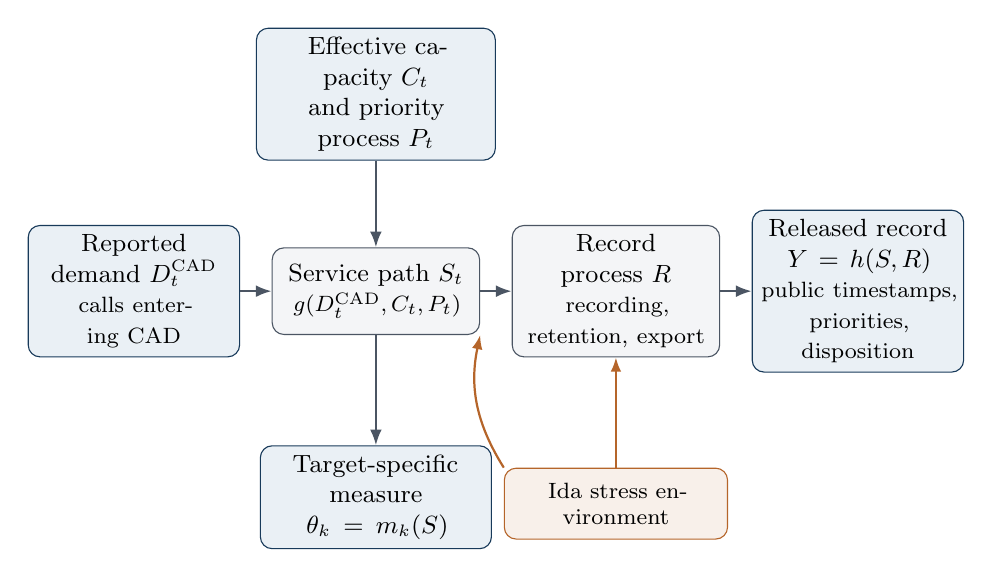
\begin{tikzpicture}[
  node distance=5mm and 4mm,
  box/.style={draw=BelandBlue,rounded corners=1.5mm,fill=BelandBlueLight,minimum height=11mm,text width=2.45cm,align=center,font=\small},
  latent/.style={draw=BelandGray,rounded corners=1.5mm,fill=BelandLightGray,minimum height=11mm,text width=2.4cm,align=center,font=\small},
  arrow/.style={-{Latex[length=2mm]},thick,draw=BelandGray}
]
\node[box] (call) {Reported demand $D_t^{\mathrm{CAD}}$\\\footnotesize calls entering CAD};
\node[latent,right=of call] (ops) {Service path $S_t$\\\footnotesize $g(D_t^{\mathrm{CAD}},C_t,P_t)$};
\node[latent,right=of ops] (record) {Record process $R$\\\footnotesize recording, retention, export};
\node[box,right=of record] (public) {Released record $Y=h(S,R)$\\\footnotesize public timestamps, priorities, disposition};
\draw[arrow] (call)--(ops);
\draw[arrow] (ops)--(record);
\draw[arrow] (record)--(public);
\node[above=11mm of ops,box,text width=2.8cm] (inputs) {Effective capacity $C_t$\\and priority process $P_t$};
\draw[arrow] (inputs)--(ops);
\node[below=14mm of ops,box,text width=2.7cm] (target) {Target-specific measure\\$\theta_k=m_k(S)$};
\draw[arrow] (ops)--(target);
\node[below=14mm of record,draw=BelandOrange,rounded corners=1.5mm,fill=BelandOrange!10,minimum height=9mm,text width=2.6cm,align=center,font=\footnotesize] (shock) {Ida stress environment};
\draw[-{Latex[length=1.8mm]},BelandOrange,thick] (shock.north) -- (record.south);
\draw[-{Latex[length=1.8mm]},BelandOrange,thick] (shock.north west) to[bend left=22] (ops.south east);
\end{tikzpicture}
\caption{Workload produces the service path; the record process produces the public observation. Target-specific witnesses establish which service measures the observation supports.}
\label{fig:chain}
\end{figure}

\section{Economic and empirical background}

Police performance is multidimensional, and administrative convenience is a weak basis for choosing a metric \citep{MooreBraga2004,TiwanaBassFarrell2015}. More generally, public-sector metrics can redirect effort toward recorded targets and alter the records used for accountability \citep{CourtyMarschke1997,Eckhouse2022}. For domestic and family violence, \citet{RollingsTaylor2008} propose measures of recording accuracy, repeat attendance, repeat offending, charging, information supplied to responders, and victim satisfaction. EIGE likewise organizes police and justice data around thirteen IPV indicators and comparable administrative definitions \citep{EIGE2023}. These studies define substantive targets. The present paper asks which targets can be recovered from a public CAD release.

Responsiveness illustrates the issue. Faster police arrival can affect clearance and injury outcomes \citep{BlanesKirchmaier2018,DeAngeloTogerWeisburd2023}. Using more than 2.7 million California fire-service incidents, \citet{BrentBeland2020} show that traffic congestion slows first responders and increases damages; their linked operational data make clear how economically consequential a valid response clock can be. Yet response time varies across reporting, dispatch, travel, and combined clocks, and the literature uses heterogeneous priority definitions and call populations \citep{VerlaanRuiter2023}. Rich internal data can link staffing, call volume, proactive work, priority, and response times \citep{MourtgosAdamsNix2024}. A public release that omits the queue, availability, or a qualified endpoint supports a narrower statistic.

The DV literature further separates reported demand from the underlying phenomenon. Calls, incidents, arrests, hotline contacts, and hospital records can move differently during the same disruption \citep{LeslieWilson2020,BullingerCarrPackham2021,MillerSegalSpencer2022,MillerSegalSpencer2024}. Disaster studies using community, postpartum, displaced-population, and adult survey samples report post-disaster associations among hurricane exposure, partner conflict or violence, and mental-health outcomes \citep{AnastarioShehabLawry2009,SchumacherEtAl2010,HarvilleTaylorTesfai2011,FirstEtAl2022}. Those studies motivate the substantive importance of a disaster-period DV measurement design, but they do not validate public CAD timestamps, identify an Ida effect on reported DV calls, or resolve selection into police records. Police composition can affect reporting \citep{MillerSegal2019}, while stable identifiers permit linkage from police reports to later economic outcomes \citep{AdamsHuttunenNixZhang2024}. This paper therefore targets performance conditional on a reported DV-related call entering CAD.

Administrative records reflect selection, classification, and linkage. Reporting, coding, and processing create successive gates \citep{KlingerBridges1997,BoivinCordeau2011,BoivinOuellet2014,SimpsonOrosco2021,KnoxLoweMummolo2020}. Call-takers assign categories and priorities before resources are deployed \citep{Pandey2025}. Fragmented DV systems and inconsistent identifiers complicate links among incidents, reports, referrals, and follow-up \citep{Phoenix2023,VomfellPovala2023}. Changes in incentives can alter registered crime \citep{AhmedLatifVyborny2026}. The measurement design must therefore describe how an operational stage becomes an observed record.

Econometric work provides the corresponding identification logic. Classical identification asks whether the observable distribution distinguishes the underlying structure \citep{KoopmansReiersol1950,Rothenberg1971,Lewbel2019}. Partial identification retains the complete set of observationally equivalent target values when it does not \citep{Manski1989,Manski1990,Manski2003,Molinari2020}. Measurement error in nonlinear settings generally requires auxiliary measurements, instruments, validation data, or explicit restrictions \citep{ChenHongNekipelov2011}. Administrative sources can measure a different concept or contain their own linkage and classification errors \citep{KapteynYpma2007}. \citet{DominitzSherman2006} derive sharp bounds on school-performance measures when an administrative verification indicator is imperfect; their measure-specific treatment of validity is especially close to the present application. Communicating the resulting nonsampling and conceptual uncertainty is part of valid official measurement \citep{Manski2015}.

Two further connections organize the witness analysis. \citet{Blackwell1953} compares information structures by the decisions they support, while \citet{MastenPoirier2020} locates boundaries at which conclusions cease to survive relaxed assumptions. Here, each administrative witness refines the feasible set of operational paths for a declared performance target. Sufficiency is reached when the target's identified set meets a prespecified precision; one-at-a-time removal establishes whether every retained witness is necessary. The resulting inclusion-minimal bundle is a target-specific release design rather than a universal ranking of data fields.

Economists also use disasters to reveal system dependencies that routine variation leaves hidden. The Great East Japan Earthquake exposed propagation through directly observed firm networks \citep{CarvalhoNireiSaitoTahbazSalehi2021}; hurricanes and outages reveal payment resilience by combining transactions, outages, surveys, and experimental evidence \citep{AlvarezArgenteVanPatten2026}. Environment comparisons can also test whether a statistical relationship remains invariant, although causal interpretation requires additional structural assumptions \citep{PetersBuhlmannMeinshausen2016}. BELAND-PLUS uses Ida at the diagnostic stage: the event tests stability of the released record, while operational witnesses determine the performance measure.

Partial identification supplies the formal response. Missing outcomes yield sharp regions, restrictions on misclassification can tighten them, and additional evidence or restrictions contract the set of observationally equivalent values \citep{Manski1990,Manski2003,HorowitzManski1995,Molinari2008,Molinari2020,Tamer2010}. BELAND-PLUS applies that logic to the measurement stage itself. Ida establishes the empirical relevance of the problem; the DV chain defines the candidate functionals and the witnesses that contract their identified sets.

\section{Institutional setting and research design}

\subsection{Hurricane Ida as a system-level stress test}

Hurricane Ida made landfall in Louisiana on 29 August 2021. The Office of the Independent Police Monitor documented twelve-hour police shifts, a period when 911 dispatch was down, anti-looting deployments, and a citywide curfew during the event \citep{OIPM2021}. Reporting, police operations, and record production were therefore exposed to simultaneous stress. This is precisely what makes Ida informative as a measurement test: it can reveal whether relationships among public fields remain stable when the system producing them is under unusual strain.

Ida is the test bed. The design uses its documented operational conditions to probe the public measurement layer; the observed topology remains compatible with several operational and record-production pathways.

The chronology is post-anchor prospective, not a pre-Ida preregistration. Ida was selected as the focal stress-test anchor before this reference-calibration stage; the three reference universes, estimator, eligibility rules, thinning rule, interval optimization, placebos, and stop rules were then frozen before the pseudo-event reference outcomes were examined.

\subsection{Why an all-call stress test informs DV measurement}

The identified-set logic can be written from the schema alone. Ida adds the empirical premise that makes the exercise consequential: the shared public observation layer actually moved outside its frozen reference class under system stress. The result replaces a generic warning about administrative data with a measured failure of stability in the fields later used for crime-specific performance analysis.

The empirical analysis uses all reported calls because every downstream call-type measure inherits that CAD layer. A DV labeling rule changes the analytic population, while its priorities, timestamps, dispositions, and links still pass through the tested record-production system. The transfer is therefore a measurement requirement. Each DV measure must establish its denominator, labeling rule, clock, endpoint selection, and lineage. The system-level estimates supply no DV-specific magnitude.

\subsection{Making the public record's shape measurable}

The analysis uses the official 2021 New Orleans Calls for Service file \citep{DataNOLA2021}. The denominator is the frozen public-created-call universe used throughout the project. For record $i$, define
\begin{align}
D_i&=\ind\{\text{a valid public dispatch field is present}\},\\
A_i&=\ind\{\text{a valid public arrival field is present}\}.
\label{eq:DA}
\end{align}
The two indicators generate four mutually exclusive public record states:

\begin{table}[t]
\centering
\caption{Public field-presence states}
\label{tab:states}
\begin{tabularx}{\textwidth}{@{}c cc X@{}}
\toprule
State & Dispatch field & Arrival field & Safe interpretation \\
\midrule
$\Jzerozero$ & absent & absent & neither public field is present \\
$\Jzeroone$ & absent & present & arrival field is present; dispatch field is absent \\
$\Jonezero$ & present & absent & dispatch field is present; arrival field is absent \\
$\Joneone$ & present & present & both public fields are present \\
\bottomrule
\end{tabularx}
\begin{minipage}{0.96\textwidth}\footnotesize
These states record public field presence. Physical-stage status requires a separate operational bridge.
\end{minipage}
\end{table}

Exactly one state is realized for every record, so the state shares sum to one. This simplex identity is central: when the share of $\Joneone$ falls, the mass must move to one or more other public states. The analysis is therefore about redistribution within the public record, not simply about a count declining.

\subsection{Event window and time bins}

The Ida window runs from 29 August 2021 at 00:00 through 3 September at 00:00 local time. It is divided prospectively into ten twelve-hour bins. To avoid unexplained internal labels, the paper reports calendar time directly; the technical labels are retained only for reproducibility. Each bin indexes when a cohort's call record was created; field states are taken from the eventual released record. The figures are therefore not contemporaneous snapshots of physical dispatch or arrival at that clock time.

\begin{table}[H]
\centering
\caption{Calendar interpretation of the focal bins}
\label{tab:bins}
\begin{tabularx}{\textwidth}{@{}l l X@{}}
\toprule
Technical bins & Calendar interval & Role in the descriptive result \\
\midrule
B1 & 29 Aug., 00:00--12:00 & opening interval; not among the nine threshold-exceeding cells \\
B2--B5 & 29 Aug., 12:00--31 Aug., 12:00 & earlier pattern: lower $\Joneone$ share \\
B6--B7 & 31 Aug., 12:00--1 Sep., 12:00 & later pattern: lower $\Joneone$ and higher $\Jzeroone$ \\
B8 & 1 Sep., 12:00--2 Sep., 00:00 & negative $\Joneone$ tail \\
B9--B10 & 2 Sep., 00:00--3 Sep., 00:00 & no cell exceeds the common threshold \\
\bottomrule
\end{tabularx}
\end{table}

\subsection{Standardized event--reference contrasts}

Within stratum $s$, time bin $t$, and state $j$, let $p^{\E}_{jst}$ and $p^{\R}_{jst}$ denote the event and reference shares. Using the frozen reference-derived common-support weights $\omega^\R_{st}$, the standardized event--reference contrast is
\begin{equation}
\Delta_{j,t}=\sum_{s\in\mathcal S_t}\omega^\R_{st}
\left(p^{\E}_{jst}-p^{\R}_{jst}\right),
\qquad
\sum_{s\in\mathcal S_t}\omega^\R_{st}=1.
\label{eq:delta}
\end{equation}
Because the four state shares sum to one,
\begin{equation}
\Delta_{00,t}+\Delta_{01,t}+\Delta_{10,t}+\Delta_{11,t}=0.
\label{eq:simplex}
\end{equation}
The primary topology matrix keeps the three independent coordinates $(\Delta_{01,t},\Delta_{10,t},\Delta_{11,t})$ for the ten bins.

\subsection{Benchmarking rarity against frozen reference windows}

The topology score measures how closely any authorized restricted-support representation can approximate the full three-coordinate path while respecting its support envelope. Let $G$ be the $10\times3$ contrast matrix and $\mathcal X$ the frozen finite set of authorized support triples. The full score can be written compactly as
\begin{equation}
U_{\mathrm{full}}(G)=
\min_{X\in\mathcal X}\max_{j\in\{01,10,11\}}
\min_{\beta_j}\norm{g_j-X\beta_j}_{\infty},
\label{eq:score_simple}
\end{equation}
subject to the rowwise capacity-envelope restrictions defined in the mathematical appendix. A larger score means that the best authorized representation leaves a larger maximum cell discrepancy. The score is a geometric measure of public-record fit.

The same estimator is applied to every qualified reference window. We report interval separation, the complete reference distribution, and the add-one reference fraction $r/(R+1)$ as descriptive measures of reference rarity.

\section{Empirical results}

The stress test must establish more than an unusual average. It asks whether Ida lies outside the range of the same measurement applied to qualified reference windows, whether the public-record shape changes during the event, and whether the later movement is merely a change in recorded-disposition mix. The three results below answer those questions in sequence.

\subsection{Ida is reference-extreme}

Ida's locked score interval is
\begin{equation}
U_{\mathrm{full}}(G_{\Ida})\in
[0.250734484671,\,0.250734494671].
\end{equation}
No reference interval overlaps it. Ida's score exceeds the score intervals of all 217 full qualified reference windows, all 153 stage-era-matched windows, and all 86 same-season-stage windows. The corresponding add-one reference fractions are $1/218$, $1/154$, and $1/87$.

\begin{figure}[t]
\centering
\begin{tikzpicture}
\begin{axis}[
  width=0.90\textwidth,height=6.0cm,
  xmin=0,xmax=222,ymin=0,ymax=0.27,
  xlabel={Qualified reference windows, ordered by upper score endpoint},
  ylabel={$U_{\mathrm{full}}$ score},
  axis x line*=bottom,axis y line*=left,
  grid=major,grid style={BelandLightGray},
  tick label style={font=\small},label style={font=\small},
  legend style={draw=none,font=\small,at={(0.02,0.98)},anchor=north west}
]
\addplot[only marks,mark=*,mark size=1.35pt,draw=BelandBlue,fill=BelandBlue]
  table[x=rank,y=U_full_upper,col sep=comma] {reference_score_distribution_r13.csv};
\addplot[only marks,mark=diamond*,mark size=3.2pt,draw=BelandOrange,fill=BelandOrange]
  coordinates {(218,0.250734494671)};
\legend{217 reference upper endpoints,Ida upper endpoint}
\end{axis}
\end{tikzpicture}
\caption{Complete distribution of the 217 full-qualified reference score upper endpoints and the Ida upper endpoint. The narrow score intervals do not overlap: the largest reference upper endpoint is $0.2125162$, below the Ida lower endpoint $0.2507345$.}
\label{fig:rank}
\end{figure}

The largest reference upper endpoint is approximately $0.2125$, leaving a minimum interval separation of about $0.0382$ from Ida. This separation is more informative than the narrower fact that Ida lies just above the frozen M7A restricted-support exclusion threshold of $0.25$. The threshold is a prespecified model-fit boundary; the empirical rank comparison is invariant to it.

\subsection{The timing placebo does not support precise institutional alignment}

The placebos distinguish topological rarity from a timing or mechanism claim. Against three frozen unlabeled duration- and mass-matched patterns, the aligned structural library has an advantage interval of $[0.2045072115,\,0.2045072215]$. In the separate zero-padded shift exercise, however, the Ida alignment-advantage interval is $[-0.1137314286,\,-0.0975331874]$: at least one arbitrary translation fits better than the documented alignment. The evidence therefore supports an unusual released-record shape, but not precise alignment with the curfew, outages, or another institutional mechanism.

\subsection{The eventual public-state configuration changes across later call-creation cohorts}

A cell is classified as unusually large when its absolute contrast exceeds the 95th percentile of the reference-window maximum absolute cell contrast,
\begin{equation}
c_{0.95}=0.209397476359.
\end{equation}
Nine bin--state cells exceed this common threshold. The pattern is easier to understand in calendar time than through technical bin labels:

\begin{itemize}
\item From the afternoon of 29 August through the morning of 31 August, the abnormal cells are reductions in $\Joneone$, the state in which both public fields are present.
\item From the afternoon of 31 August through the morning of 1 September, $\Joneone$ remains sharply lower, while $\Jzeroone$---arrival present but dispatch absent---becomes sharply higher.
\item During the afternoon and evening of 1 September, the negative $\Joneone$ contrast remains above the threshold, but $\Jzeroone$ no longer does.
\end{itemize}

\begin{figure}[t]
\centering
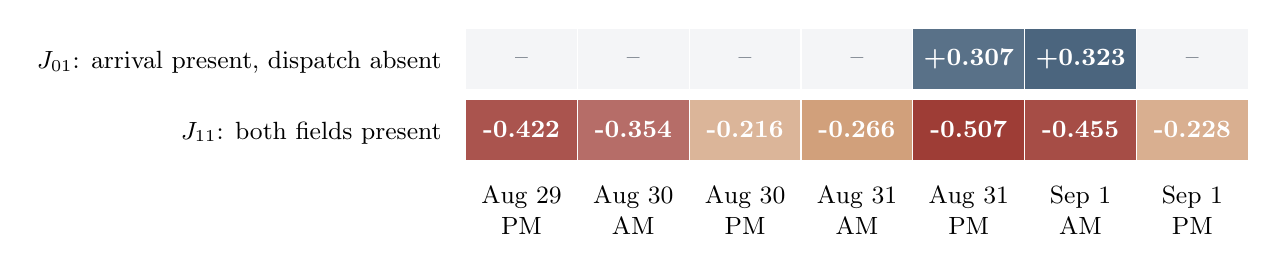
\begin{tikzpicture}[font=\small]
\def\cellw{1.42}
\def\cellh{0.78}
\node[anchor=east] at (-0.18,0) {$\Joneone$: both fields present};
\node[anchor=east] at (-0.18,0.9) {$\Jzeroone$: arrival present, dispatch absent};
\foreach \x/\lab in {0/{Aug 29\\PM},1/{Aug 30\\AM},2/{Aug 30\\PM},3/{Aug 31\\AM},4/{Aug 31\\PM},5/{Sep 1\\AM},6/{Sep 1\\PM}} {
  \node[align=center,anchor=north] at ({\x*\cellw+0.5*\cellw},-0.56) {\lab};
}
% J11 row
\foreach \x/\v/\col in {0/-0.422/BelandRed!88,1/-0.354/BelandRed!75,2/-0.216/BelandOrange!48,3/-0.266/BelandOrange!62,4/-0.507/BelandRed,5/-0.455/BelandRed!92,6/-0.228/BelandOrange!52} {
  \fill[\col] ({\x*\cellw},-0.35) rectangle ++(\cellw,\cellh);
  \draw[white!35] ({\x*\cellw},-0.35) rectangle ++(\cellw,\cellh);
  \node[text=white,font=\small\bfseries] at ({\x*\cellw+0.5*\cellw},0.04) {\v};
}
% J01 row
\foreach \x in {0,1,2,3,6} {
  \fill[BelandLightGray] ({\x*\cellw},0.55) rectangle ++(\cellw,\cellh);
  \draw[white] ({\x*\cellw},0.55) rectangle ++(\cellw,\cellh);
  \node[text=BelandGray] at ({\x*\cellw+0.5*\cellw},0.94) {--};
}
\foreach \x/\v/\col in {4/+0.307/BelandBlue!72,5/+0.323/BelandBlue!78} {
  \fill[\col] ({\x*\cellw},0.55) rectangle ++(\cellw,\cellh);
  \draw[white!35] ({\x*\cellw},0.55) rectangle ++(\cellw,\cellh);
  \node[text=white,font=\small\bfseries] at ({\x*\cellw+0.5*\cellw},0.94) {\v};
}
\end{tikzpicture}
\caption{The nine threshold-exceeding public-record cells. Values are event-minus-reference probability-point contrasts; a dash marks a cell below the common threshold. The figure describes public field configurations.}
\label{fig:heatmap}
\end{figure}

The result is a redistribution statement: one public state falls while another rises. Its generating pathway remains set-valued.

\subsection{The later shift occurs within recorded dispositions}

The next question is whether the late pattern could arise solely because the mix of dispositions changed. Restrict attention to arrival-observed records, $\Jzeroone+\Joneone$. For disposition $r$ and population $z\in\{\E,\R\}$, let
\begin{equation}
q^z_r=\Prob(D=1\given A=1,R=r,z),
\qquad
\pi^z_r=\Prob(R=r\given A=1,z).
\end{equation}
The aggregate dispatch-field share among arrival-observed records is $q^z_{\mathrm{all}}=\sum_r\pi^z_rq^z_r$. The exact symmetric Kitagawa identity is
\begin{align}
q^\E_{\mathrm{all}}-q^\R_{\mathrm{all}}
={}&\sum_r\frac{q^\E_r+q^\R_r}{2}(\pi^\E_r-\pi^\R_r) \notag\\
&+\sum_r\frac{\pi^\E_r+\pi^\R_r}{2}(q^\E_r-q^\R_r).
\label{eq:kitagawa}
\end{align}
The first term is the recorded-disposition composition component. The second is the within-disposition component.

\begin{figure}[t]
\centering
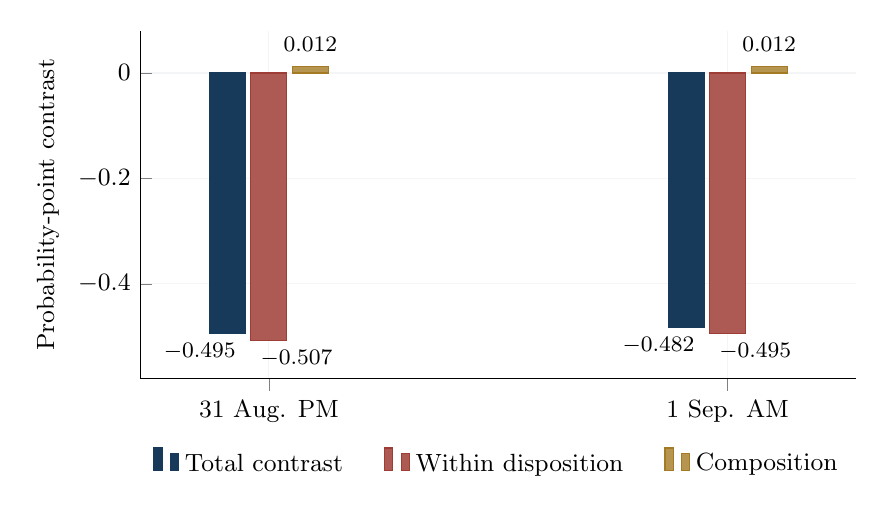
\begin{tikzpicture}
\begin{axis}[
  width=0.88\textwidth,height=6.0cm,
  ybar,bar width=13pt,
  ymin=-0.58,ymax=0.08,
  ylabel={Probability-point contrast},
  symbolic x coords={31 Aug. PM,1 Sep. AM},xtick=data,
  legend style={at={(0.5,-0.18)},anchor=north,legend columns=3,draw=none,font=\small,
    /tikz/every even column/.append style={column sep=0.45cm}},
  legend cell align={left},
  axis x line*=bottom,axis y line*=left,
  grid=major,grid style={BelandLightGray},
  tick label style={font=\small},label style={font=\small},
  enlarge x limits=0.28
]
\addplot[fill=BelandBlue,draw=BelandBlue,
  nodes near coords={\pgfmathprintnumber[fixed,precision=3]{\pgfplotspointmeta}},
  every node near coord/.append style={font=\footnotesize,xshift=-10pt}]
  coordinates {(31 Aug. PM,-0.4950) (1 Sep. AM,-0.4824)};
\addplot[fill=BelandRed!85,draw=BelandRed,
  nodes near coords={\pgfmathprintnumber[fixed,precision=3]{\pgfplotspointmeta}},
  every node near coord/.append style={font=\footnotesize,xshift=10pt}]
  coordinates {(31 Aug. PM,-0.5069) (1 Sep. AM,-0.4946)};
\addplot[fill=BelandGold!80,draw=BelandGold,
  nodes near coords={\pgfmathprintnumber[fixed,precision=3]{\pgfplotspointmeta}},
  every node near coord/.append style={font=\footnotesize,yshift=2pt}]
  coordinates {(31 Aug. PM,0.0119) (1 Sep. AM,0.0123)};
\legend{Total contrast,Within disposition,Composition}
\end{axis}
\end{tikzpicture}
\caption{Exact accounting decomposition of the late aggregate shift. The small positive composition term has the opposite sign from the negative total contrast.}
\label{fig:kitagawa}
\end{figure}

For 31 August afternoon/evening, the total contrast is $-0.4950$, the composition component is $+0.0119$, and the within-disposition component is $-0.5069$. For 1 September morning, the corresponding values are $-0.4824$, $+0.0123$, and $-0.4946$. The within-disposition component accounts for the direction and almost all of the magnitude of the aggregate shift in this decomposition.

The sign pattern strengthens the accounting result. For Gone on Arrival (GOA), Report to Follow (RTF), and Necessary Action Taken (NAT), $\Delta H_{01,r}>0$ while $\Delta H_{11,r}<0$ in both late bins. A composition-only explanation based on the observed final-disposition mix among arrival-observed records requires matching signs, so the six prespecified cells rule out that explanation alone. This does not rule out selection into the arrival-observed set, unobserved composition, within-category heterogeneity, semantic drift, or alternative service and record-production pathways.

\begin{table}[H]
\centering
\caption{Within-disposition change in the public dispatch-field share among arrival-observed records}
\label{tab:disp}
\begin{tabular}{@{}lrrr@{}}
\toprule
Calendar bin & GOA & RTF & NAT \\
\midrule
31 Aug., 12:00--24:00 & $-0.440$ & $-0.567$ & $-0.532$ \\
1 Sep., 00:00--12:00 & $-0.265$ & $-0.459$ & $-0.649$ \\
\bottomrule
\end{tabular}
\begin{minipage}{0.94\textwidth}\footnotesize
Each value is an event-minus-reference contrast in the public dispatch-field share among arrival-observed records within the named recorded disposition. GOA is Gone on Arrival; RTF is Report to Follow; NAT is Necessary Action Taken. All three are administrative categories.
\end{minipage}
\end{table}

Table~\ref{tab:disp} reports conditional-share contrasts, whereas Appendix Section~5.1 factors the corresponding joint masses as $H_{11}=mq$ and $H_{01}=m(1-q)$; Appendix Table~4 reports their contrasts. The tables therefore describe linked but distinct quantities: the first localizes conditional public-field movement, while the second supplies the sign witnesses used to exclude composition-only.

Together, the results establish an extreme, time-structured change in the public administrative trace, including movement within recorded dispositions. They show that relationships among released fields were not mechanically stable during Ida; they do not establish which operational or record-production pathway changed.

This is the empirical bridge to DV measurement. A DV label selects records after they have passed through the same field-production system. The performance question then becomes measure-specific: which operational functionals retain a unique interpretation after that selection?

The all-call result neither estimates DV demand nor implies that every DV measure fails. It establishes a common observation-layer problem. The DV application determines which targets survive that problem and which require additional evidence.

\begin{resultbox}
\textbf{Stress-test implication.} Ida establishes instability in the released measurement product. Operational interpretation requires a separate identified-set analysis for each downstream measure.
\end{resultbox}

\section{From the Ida diagnostic to measure-specific identification}

The empirical statistic and the performance target are different mathematical objects. The stress-test statistic is a function of released records,
\begin{equation}
T(Y):=U_{\mathrm{full}}(G(Y)).
\label{eq:diagnostic}
\end{equation}
Its reference rank establishes that Ida's public-field path is unusual within the frozen comparison design. A candidate performance target instead depends on the latent operational path $S$.

Let $W$ denote the available semantic and operational witnesses, and let $\mathcal C(W)$ collect the paths and recording processes consistent with those witnesses. For candidate measure $\theta_k=m_k(S)$, define
\begin{equation}
\mathcal I_k(Y,W)
=
\left\{m_k(S):Y=h(S,R),\ (S,R)\in\mathcal C(W)\right\}.
\label{eq:measure_set}
\end{equation}
The measure is directly supportable when this set is a singleton, bounded when it is informative but non-singleton, selected when its observed version conditions on a narrower risk set, and unavailable when current evidence leaves the target unrestricted or undefined. New witnesses contract $\mathcal C(W)$ and therefore weakly contract $\mathcal I_k(Y,W)$.

\subsection{Internal stage occurrence versus public capture}

Suppose future semantic evidence established a valid direct bridge between a qualified internal administrative dispatch event and the public dispatch field. Let
\begin{equation}
q^{\mathrm{pub}}=\Prob(D_{\mathrm{pub}}=1\given A_{\mathrm{pub}}=1,R=r,t),
\end{equation}
\begin{equation}
u=\Prob(U_{\mathrm{dispatch}}=1\given A_{\mathrm{pub}}=1,R=r,t),
\end{equation}
\begin{equation}
\chi=\Prob(D_{\mathrm{pub}}=1\given U_{\mathrm{dispatch}}=1,A_{\mathrm{pub}}=1,R=r,t).
\end{equation}
Under exact nesting, the observed public share factorizes as
\begin{equation}
q^{\mathrm{pub}}=u\chi.
\label{eq:product}
\end{equation}
For any $0<q^{\mathrm{pub}}<1$, the identified set is
\begin{equation}
\Iset(u,\chi\given q^{\mathrm{pub}})
=\{(u,q^{\mathrm{pub}}/u):u\in[q^{\mathrm{pub}},1]\}.
\label{eq:hyperbola}
\end{equation}
The same public value is compatible with perfect public capture and a lower internal-stage prevalence, complete internal-stage prevalence and imperfect public capture, and every intermediate combination.

\begin{figure}[t]
\centering
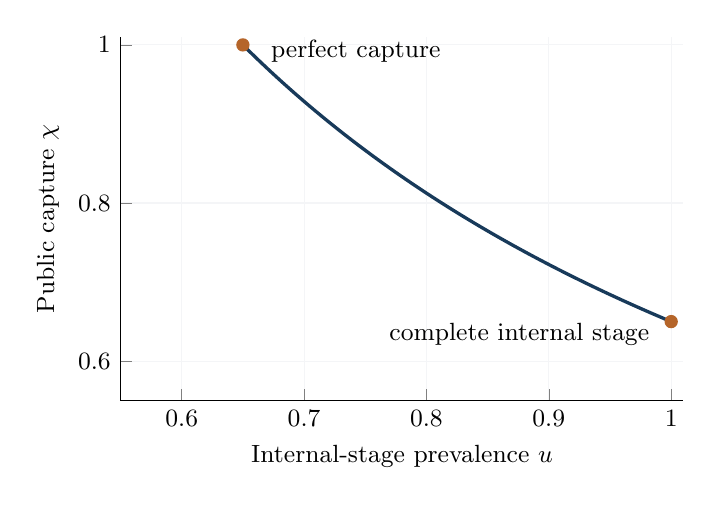
\begin{tikzpicture}
\begin{axis}[
  width=0.72\textwidth,height=6.2cm,
  xmin=0.55,xmax=1.01,ymin=0.55,ymax=1.01,
  xlabel={Internal-stage prevalence $u$},
  ylabel={Public capture $\chi$},
  axis x line*=bottom,axis y line*=left,
  grid=major,grid style={BelandLightGray},
  tick label style={font=\small},label style={font=\small},
  legend style={draw=none,font=\small,at={(0.98,0.05)},anchor=south east}
]
\addplot[domain=0.65:1,samples=150,very thick,BelandBlue] {0.65/x};
\addplot[only marks,mark=*,mark size=2.2pt,BelandOrange] coordinates {(0.65,1) (1,0.65)};
\node[anchor=south west,font=\small] at (axis cs:0.665,0.965) {perfect capture};
\node[anchor=north east,font=\small] at (axis cs:0.99,0.66) {complete internal stage};
\end{axis}
\end{tikzpicture}
\caption{Illustrative product identified set for $q^{\mathrm{pub}}=0.65$. Observing the product selects a curve of internal-stage and capture values. The value $0.65$ is illustrative.}
\label{fig:hyperbola}
\end{figure}

The product identifies a curve rather than a unique pair. Joint public--internal counts would separate internal-stage prevalence from public capture. This example is a special case of \cref{eq:measure_set}: timestamp precision does not establish the mapping from a public field to the operational stage it is intended to measure.

A DV labeling rule restricts the analytic population but leaves the observation map unchanged. The DV results below are derived by applying \cref{eq:measure_set} to that selected chain. They are measurement results, not an empirical DV subset analysis.

\subsection{Queue, availability, priority history, and continuity}

Queue dynamics live on a different denominator. A qualified stock-flow identity would have the form
\begin{equation}
Q_{t+1}=Q_t+I_t-O_t-X_t,
\label{eq:queue}
\end{equation}
where $Q_t$ is calls holding, $I_t$ is inflow, $O_t$ is ordinary outflow, and $X_t$ is another qualified exit. Populating the identity requires calls-holding stocks, inflows, exits, and realized availability. Ordered priority histories and follow-up states add the remaining transitions.

Endpoint timestamps omit the stock waiting, the resources available, and the sequence of priority and exit changes. The product and queue examples show how each performance target selects its own denominator, clock, and witness requirements.

\subsection{Operational and record-production friction}

The observation map separates two forms of friction. Operational friction changes the service path through congestion, unit availability, assignment, handoffs, or follow-up. Record-production friction changes how those stages are classified, overwritten, retained, linked, or exported. Both can produce gaps in public timestamps or changes in public-state composition.

The Ida pattern is compatible with either source, or with both operating together. The diagnostic supplies no probability ordering over them. Target-specific witnesses localize the ambiguity: holding and availability histories recover operational congestion; joint public--internal counts recover capture; retained lineage reveals where records cease to share a denominator. A better release therefore improves measurement by contracting the relevant identified set. Whether a reform also reduces operational friction is a separate evaluative question.

\section{From identified sets to admissible measures}

Equation~\ref{eq:measure_set} turns five design choices into an admissibility test: labeling rule, denominator, operational clock, endpoint selection, and stage lineage. Equation~\ref{eq:product} motivates lineage; Equation~\ref{eq:queue} motivates stocks and transitions. Ida makes these choices empirically consequential because the shared public trace changed while its generating pathway remained set-valued.

Directly supportable administrative measures are functions of the released file under an explicit rule and denominator. Bounds propagate unresolved labels or missing outcomes. Selected measures describe the risk set on which their endpoints are observed. Measures requiring absent clocks, states, or links become available when the corresponding witnesses enter $W$.

Responsiveness requires a time origin, endpoint, and population at risk. Prioritization requires an ordered history when priorities change. Follow-through requires links from CAD to the applicable downstream stage, such as EPR production, program referral, or a policy-defined callback. A recorded disposition can mark an administrative branch, including GOA, while later duties require their own evidence.

NOPD policy anticipates assigned units, dispatch, arrival, return-to-service, and disposition in the communications record \citep{NOPDManual}. Later oversight and court-directed reforms identify response time, calls holding, priority changes, officer availability, callbacks, accessibility, and data quality as operational objects \citep{SustainmentPlan2024,CourtOrder2025,OIPM2022,OIPM2026}. These documents establish why each object matters, while the public CAD files do not record callback eligibility or completion. Empirical measurement requires period-specific values and retained lineage.

Before applying the framework to reported DV-related calls, one further question is necessary: did later public-data enrichment supply the missing clocks and links, making the Ida lesson specific to the 2021 data regime?

\section{Do newer public data close the measurement gap?}

We retrieved and froze the official 2025 and 2026 Calls for Service datasets, their metadata and dictionaries, the current response-time dashboard model, current response policies, and the 2025 Electronic Police Report metadata \citep{DataNOLA2025,DataNOLA2026,NOPDPolicy2025,NOPDAPR2024,NOPDResponseDashboard2026}. The comparison evaluates public measurement regimes.

The newer regime adds machine-queryable derived fields, including a candidate en-route duration and multiple dispositions. Current policies also clarify priority ordering, alternate response, policy-defined callbacks, and return-to-queue rules. The annual raw schema retains the 2021 structure: initial and recorded signal/priority endpoints, create/dispatch/arrival/closure timestamps, final disposition, and self-initiation.

The structural witnesses remain separate. Public documentation leaves the derived clocks, ordering, multiplicity, overwrite behavior, and historical continuity unresolved. Calls holding, realized unit availability, timestamped priority histories, applicable callback or fallback states, and public--internal dispatch lineage require internal aggregate evidence.

\begin{table}[H]
\centering
\caption{Post-Ida public enrichment and the remaining structural boundary}
\label{tab:m8p}
\begin{tabularx}{\textwidth}{@{}l X X@{}}
\toprule
Object & Public improvement by 2025--2026 & Remaining boundary \\
\midrule
Internal/public dispatch bridge & more public analytical surfaces and a 2025 CAD--EPR item link & qualified internal dispatch event and field-lineage map needed \\
Queue and availability & endpoint durations and response-time summaries & calls-holding stock, unit-status history, and realized availability needed \\
Priority & initial/recorded endpoints, change flags, and clearer current policy & ordered event history, actor, reason, and overwrite trail needed \\
Continuity and fallback & current policies describe alternate routes and policy-defined callbacks & realized uptime, fallback activation, and applicable callback-execution state needed \\
\bottomrule
\end{tabularx}
\end{table}

The current-data audit illustrates endpoint selection. The 2025 file contains 152,701 records with an arrival field but no dispatch field; the 2026 snapshot contains 97,573. A dispatch-to-arrival duration excludes these arrival-observed records. Dispatch-field completeness is approximately 41.8 percent in both years. Exact initial-versus-recorded priority disagreement is 38.7 percent in 2025 and 37.1 percent in the 2026 snapshot. These all-call values establish pervasive contemporary public-field missingness and endpoint change. Their scope is the observed audit periods.

The replay sharpens the Ida lesson. Public enrichment improves description; performance measurement still requires lineage, complete clocks, and common denominators. The DV application now carries those requirements through the reporting-to-follow-up chain.

\section{Implications for a reported-DV performance study}

The framework now turns to the substantive objective. Candidate DV measures begin with the public fields tested under Ida and extend to reports and follow-up when retained links permit. The application derives each measurement status from the evidence required at its stage.

\subsection{The shared CAD layer and the reporting-to-follow-up chain}

The project's M7C selection map follows a reported DV-related call through priority, public dispatch and arrival fields, recorded disposition, Electronic Police Report (EPR) production, and possible DVU or AIR entry. The frozen machine-readable records are \path{M7C_DV_STAGE_MAP.json} and \path{M7C_FROZEN_SOURCE_INVENTORY.json}:
\begin{equation*}
\begin{aligned}
\text{reported DV-related CAD}
&\rightarrow \text{priority}
\rightarrow \text{public dispatch/arrival fields}\\
&\rightarrow \text{recorded disposition}
\rightarrow \text{EPR}
\rightarrow \text{DVU/AIR}.
\end{aligned}
\end{equation*}
Each arrow requires a retained link, and each downstream stage creates a new denominator. A DV label defines the first box. DVU audit compliance describes sampled DVU files; AIR describes an advocacy-eligible pathway after program launch. Upstream lineage is needed to express either stage as a share of reported DV-related CAD records.

\subsection{Reported demand begins at the CAD denominator}

The workload estimand begins with calls created in CAD, $D_t^{\mathrm{CAD}}$. It therefore measures reported demand recorded by the dispatch system. Help-seeking attempts that never reach the system, contacts received without a retained CAD record, and underlying DV need occupy earlier stages of the demand chain. Measuring those stages requires external access, survey, hotline, or validation evidence.

This distinction also governs interpretation of call volume. A change in released counts can reflect help-seeking, access, CAD creation, classification, retention, or the underlying phenomenon. R13.0 retains the R12 system-level Ida record-state estimates; it reports no DV call-count trend. The DV application begins at the declared CAD denominator and asks how far performance measurement can proceed from there.

\subsection{Classification defines the first denominator}

Classification defines the first denominator. The available map lacks a fully qualified, period-specific frozen signal list. A declared rule therefore places records into three groups: DV-related, other, and unresolved. The unresolved group enters the bounds directly.

Let $\mathcal L$ denote the declared labeling rule and let $C_i^{\mathcal L}\in\{1,0,U\}$ denote its three states: labeled DV-related, labeled not DV-related, and unresolved. If $N_1=\sum_i\ind\{C_i^{\mathcal L}=1\}$ and $N_U=\sum_i\ind\{C_i^{\mathcal L}=U\}$, the sharp count bound is
\begin{equation}
N_{\mathrm{DV}}^{\mathcal L}\in[N_1,\,N_1+N_U].
\label{eq:dv_bounds}
\end{equation}
For a fixed CAD denominator $N$, the corresponding share lies in $[N_1/N,(N_1+N_U)/N]$. The superscript ties the estimand to rule $\mathcal L$. Appendix Section~6.8 gives the labeling semantics and sharpness argument.

At the disposition stage, GOA is a recorded administrative branch. It becomes performance-relevant when policy attaches a specific downstream duty, such as report production or an applicable callback; completion of that duty supplies the corresponding outcome.

\subsection{Response-time selection and sharp full-denominator bounds}

Let $E_i=1$ when the timestamps required for a declared response-time clock are observed. Among records labeled DV-related under $\mathcal L$, define
\begin{equation}
\pi_E=\Prob(E=1\given C^{\mathcal L}=1),
\qquad
F_E(a)=\Prob(\tau\le a\given C^{\mathcal L}=1,E=1).
\end{equation}
The public file directly supports the selected distribution $F_E$. The desired distribution over the full declared-rule denominator is
\begin{equation}
F_\tau(a)=\pi_EF_E(a)+(1-\pi_E)F_0(a),
\end{equation}
where $F_0$ is the unobserved distribution for endpoint-missing records. Allowing $F_0(a)$ to range over $[0,1]$ gives the sharp pointwise bounds
\begin{equation}
\pi_EF_E(a)
\le F_\tau(a)\le
\pi_EF_E(a)+(1-\pi_E).
\label{eq:response_bounds}
\end{equation}
These bounds state exactly what endpoint selection costs. Qualified endpoint recovery or a defensible restriction on the missing group narrows the interval. Unresolved $U$ labels enlarge the outer set through \cref{eq:dv_bounds}.

\subsection{Priority histories and administrative follow-through}

Initial and recorded priorities reveal endpoint disagreement. If $H_i=1$ denotes at least one priority change, then
\begin{equation}
\Prob(P^0\ne P^r)
\le \Prob(H=1)\le 1.
\label{eq:priority_bounds}
\end{equation}
Ordered priority histories replace this bound with measured transitions, their timing, and their direction.

For follow-through, let $L_i=1$ indicate retained lineage from the CAD denominator to the declared follow-up stage and let $Z_i=1$ indicate completion of the specified administrative duty. Define
\begin{equation}
\pi_L=\Prob(L=1\given C^{\mathcal L}=1),
\qquad
p_L=\Prob(Z=1\given C^{\mathcal L}=1,L=1).
\end{equation}
The full-denominator completion rate $p_Z$ obeys
\begin{equation}
\pi_Lp_L
\le p_Z\le
\pi_Lp_L+(1-\pi_L).
\label{eq:follow_bounds}
\end{equation}
When lineage coverage is unavailable, the public-data set is $[0,1]$. Aggregate retained lineage identifies $\pi_L$; linked completion counts identify $p_L$ and close the remaining gap.

\subsection{What current evidence can support}

\begin{table}[H]
\centering
\caption{Measurement frontier along the reported-DV administrative chain}
\label{tab:dv_admissibility}
\begin{tabularx}{\textwidth}{@{}>{\raggedright\arraybackslash}p{2.45cm} X X@{}}
\toprule
Class & Candidate measure & Supported interpretation \\
\midrule
Directly supportable administrative measure &
Rule-defined reported-DV counts and $1/0/U$ bounds; recorded disposition composition; public-field completeness &
Functions of released fields on an explicit CAD denominator. The declared rule and unresolved class remain part of the estimand. \\
\addlinespace
Bounded or selected measure &
Response times among records with the required endpoints; initial and recorded priority endpoints; CAD--EPR key presence; DVU or AIR measures on their own denominators &
Equations~\ref{eq:response_bounds}--\ref{eq:follow_bounds} propagate endpoint and lineage coverage; downstream programs retain their selected denominators. \\
\addlinespace
Unavailable from public CAD &
Physical service stages; queue delay; realized unit availability or effective capacity; policy-defined callback completion; response quality; victim safety; true DV incidence; a unique mechanism &
Internal states, retained links, or separate outcome evidence are required to define these targets. \\
\bottomrule
\end{tabularx}
\end{table}

The table applies \cref{eq:measure_set}. Classification uncertainty produces count bounds, endpoint missingness produces selected distributions and full-denominator bounds, and downstream programs define new populations. Retained lineage places these components on a common reported-call denominator.

\subsection{Target-specific privacy-conscious witness sets}

Minimality is target-specific because each performance measure uses a different denominator, clock, or completion rule. Appendix Section~1.3 formalizes the relevant standard. Building on observational equivalence and partial identification, a witness bundle is sufficient for a declared target when it defines the risk set and contracts the target's identified set to the prespecified precision. It is inclusion-minimal when removing any member restores excess ambiguity or leaves the target undefined. We call this a target-specific witness sufficiency and necessity analysis. Minimum cost or minimum disclosure are separate implementation criteria and can select among several inclusion-minimal bundles.

Qualified period-specific DV labeling and retained event lineage form the common core. The lineage remains internal: its role is to produce reconciled aggregate cells on the same reported-call denominator. The measure-specific additions are shown in Table~\ref{tab:witness_bundles}.

\begin{table}[H]
\centering
\caption{Target-specific privacy-conscious witness bundles}
\label{tab:witness_bundles}
\begin{tabularx}{\textwidth}{@{}>{\raggedright\arraybackslash}p{2.75cm} X X@{}}
\toprule
Target & Required joint witness & Additional information for a broader target \\
\midrule
Reported-DV risk set &
Qualified period-specific labeling rule, prespecified treatment of $U$, and internal lineage capable of producing reconciled aggregate cells &
Separate validation evidence if the target changes from a declared administrative label to underlying DV status \\
\addlinespace
Receipt-to-assignment delay &
CAD receipt and first qualified assignment times for the same calls, with endpoint coverage on the full denominator &
Realized unit availability for capacity-adjusted delay or an operational explanation \\
\addlinespace
Receipt-to-qualified-arrival responsiveness &
CAD receipt and qualified operational arrival endpoints for the same calls, with endpoint coverage &
Calls-holding and availability histories when the target decomposes total time into queue and travel components \\
\addlinespace
Priority revision &
Initial priority and the complete ordered priority history, including event times and direction &
Actor and reason fields for process or rule-compliance analysis \\
\addlinespace
Administrative follow-through &
Duty eligibility, retained CAD--stage lineage, and completion status or time for the applicable downstream stage (EPR, program referral, or policy-defined callback) &
Content or quality evidence when the target extends beyond completion of the declared duty \\
\bottomrule
\end{tabularx}
\end{table}

The required evidence is joint rather than marginal. A privacy-conscious release must preserve cells such as reported-DV calls by endpoint coverage and duration bin, or eligible calls by lineage and completion status. Public event identifiers are unnecessary when the agency constructs those cells internally and applies small-cell suppression; the phrase privacy-conscious does not assert a formal privacy guarantee.

The necessity arguments clarify the boundary. Removing the labeling rule changes the reported-DV risk set. Removing lineage permits the same marginal clocks or completion totals to be matched to different CAD calls. Removing one response clock leaves duration undefined; incomplete endpoint coverage leaves a selected distribution and the bounds in \cref{eq:response_bounds}. Endpoint priorities permit offsetting changes, whereas an ordered history measures them. Follow-through requires both duty eligibility and completion on the common denominator.

Calls-holding transitions therefore belong to the minimum bundle for queue delay, while realized unit availability belongs to a capacity-adjusted target. A fully observed receipt-to-qualified-endpoint distribution uses neither. These target-complete bundles support performance measurement conditional on reported DV-related calls received by CAD. Population incidence, victim safety, and mechanism remain distinct estimands.

\subsection{A DV-specific estimator would be a new empirical extension}

A DV-subset version of the ten-bin event--reference estimator is a separate empirical extension. It requires qualified period-specific classification authority, prespecified treatment of $U$ records, support and cell-size floors, prespecified reference eligibility, and selection handling for endpoints and downstream stages. Its reference set would be requalified for the DV estimand. R13.0 reports only the frozen R12 system-level estimates.

\section{Implications for resource allocation and civilian oversight}

The witness analysis turns the measurement frontier into a release design. The same aggregate evidence serves two users. Police managers need common-denominator flows to align capacity with reported demand and locate delay. Civilian oversight needs the same flows to distinguish congestion, prioritization, endpoint coverage, and administrative follow-through.

\begin{table}[H]
\centering
\caption{A shared measurement layer for management and oversight}
\label{tab:allocation_oversight}
\begin{tabularx}{\textwidth}{@{}>{\raggedright\arraybackslash}p{3.05cm} X X@{}}
\toprule
Aggregate object & Resource-management use & Civilian-oversight use \\
\midrule
Reported calls by qualified label and priority & Describe incoming workload and priority mix & Reconcile the population used in published measures \\
\addlinespace
Calls holding and realized availability over time & Locate queue pressure and capacity constraints & Separate waiting from endpoint or recording gaps \\
\addlinespace
Receipt, assignment, and qualified endpoint distributions & Compare delay across declared stages and risk sets & Audit endpoint coverage and selected response summaries \\
\addlinespace
CAD--applicable-stage lineage and completion cells & Locate administrative attrition and follow-up workload & Verify completion rates on the original eligible-call denominator \\
\bottomrule
\end{tabularx}
\end{table}

These objects can be released as time-binned joint counts, coverage rates, transition matrices, and duration distributions with small-cell suppression. The design requires neither victim identifiers, unit identifiers, exact locations, nor live deployment information. Stable definitions, versioned labeling rules, and reconciled denominators allow managers and reviewers to reproduce each published measure.

The payoff has two stages. Better releases contract identified sets immediately, making descriptive performance measures more precise and comparable. Richer lineage can then support evaluation of staffing, dispatch, reporting, or policy-defined follow-up reforms when paired with a credible experimental or quasi-experimental design. Ida is unsuitable as an instrument for those effects because it jointly perturbed demand, operations, and recording. Its role is to reveal the measurement problem that a later causal design must first solve.

\section{Limitations}

The Ida statistic measures rarity within frozen comparison sets; the Kitagawa calculation is an accounting decomposition, and the institutional timeline supplies context. The event jointly stressed operations and record production, so the generating pathway remains set-valued. The 2025--2026 audit describes its observed public-data regime. Help-seeking, access, evacuation, mobility, holidays, weather, COVID-era conditions, redaction, and suppression can also change reported-call populations.

The DV application establishes a measurement frontier. Exact period-specific signal-list authority remains unresolved where noted, and downstream sources condition on selected populations. An empirical DV performance estimate requires qualified classification and the aggregate lineage specified above.

\section{Conclusion}

Police workload theory links reported demand, effective capacity, priorities, and service. Ida establishes that the public observation of that system can change in an extreme, structured, within-disposition way. Its score is reference-extreme, while the service and record-production paths that generated the pattern remain observationally equivalent.

The measure-specific identified set carries that finding to reported DV-related calls. Declared-rule administrative counts and $1/0/U$ bounds are directly supportable. Endpoint-observed response times describe a selected risk set, with sharp full-denominator bounds determined by coverage. Ordered histories recover priority revision. Retained CAD-to-applicable-downstream-stage lineage places administrative follow-through on the original eligible-call denominator.

Qualified labeling and privacy-conscious aggregate lineage form the common measurement core. Identified-set contraction and witness-necessity arguments then select the clocks, histories, eligibility rules, completion fields, holding stocks, and availability measures required by particular estimands. Released as suppressed aggregate joint cells, these witnesses let managers locate workload pressure and let civilian reviewers audit the same denominators and transitions.

The motivating question therefore has a conditional answer. Public CAD supports defensible administrative measures whose labels, fields, and risk sets are explicit; responsiveness, prioritization, and follow-through require the additional witnesses derived here. Those data would support an empirical DV performance study and stronger future evaluations of resource allocation. True DV incidence, victim safety, and the mechanism behind the Ida pattern remain separate targets.

\bibliographystyle{apalike}
\bibliography{references_r13_0}

\end{document}
